% \section{Loss Function}
% A loss function or cost function (sometimes also called an error function) is a function that maps an event or values of one or more variables onto a real number intuitively representing some "cost" associated with the event. An optimization problem seeks to minimize a loss function. An objective function is either a loss function or its opposite (in specific domains, variously called a reward function, a profit function, a utility function, a fitness function, etc.), in which case it is to be maximized. The loss function could include terms from several levels of the hierarchy.
% \par \vspace{1em}

% \begin{figure}
%     \centering
%     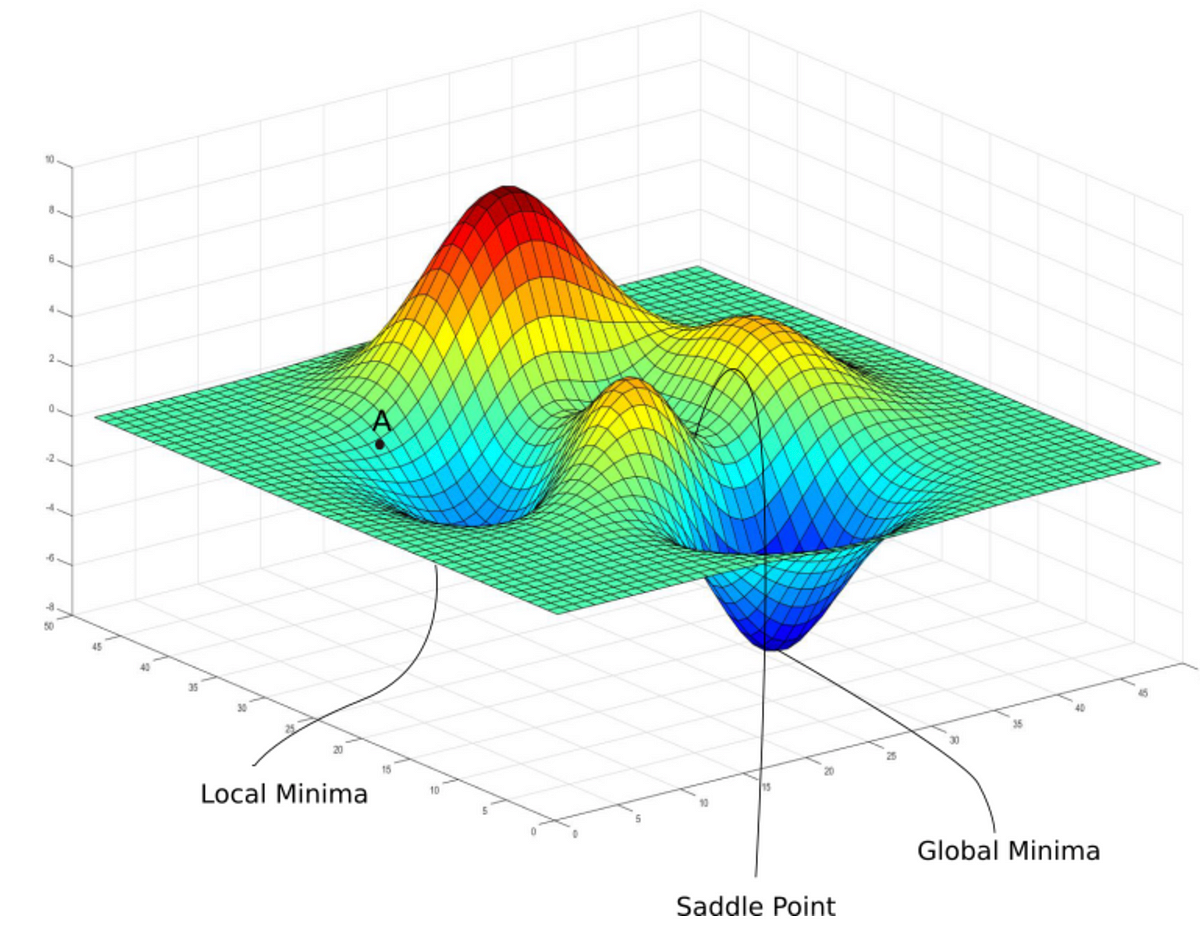
\includegraphics[width=0.75\linewidth]{graphics//chapter3/loss with local global minima.png}
%     \caption{Loss Function with a local, global and saddle point}
%     \label{fig:loss-lgs}
% \end{figure}

% \begin{figure}
%     \centering
%     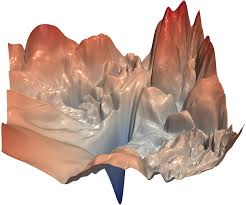
\includegraphics[width=0.75\linewidth]{graphics//chapter3/loss landscape.png}
%     \caption{Loss surface learned by neural networks }
%     \label{fig:loss-landscape}
% \end{figure}

% In statistics, typically a loss function is used for parameter estimation, and the event in question is some function of the difference between estimated and true values for an instance of data. The concept, as old as Laplace, was reintroduced in statistics by Abraham Wald in the middle of the 20th century.In the context of economics, for example, this is usually economic cost or regret. In classification, it is the penalty for an incorrect classification of an example. In actuarial science, it is used in an insurance context to model benefits paid over premiums, particularly since the works of Harald Cramér in the 1920s.In optimal control, the loss is the penalty for failing to achieve a desired value. In financial risk management, the function is mapped to a monetary loss.
%     \subsection{Mean Squared Error (MSE)}
%     The mean squared error (MSE) or mean squared deviation (MSD) of an estimator (of a procedure for estimating an unobserved quantity) measures the average of the squares of the errors i.e., the average squared difference between the estimated values and the actual value. MSE is a risk function, corresponding to the expected value of the squared error loss.The fact that MSE is almost always strictly positive (and not zero) is because of randomness or because the estimator does not account for information that could produce a more accurate estimate.In machine learning, specifically empirical risk minimization, MSE may refer to the empirical risk (the average loss on an observed data set), as an estimate of the true MSE (the true risk: the average loss on the actual population distribution).\par\vspace{1em}
%  % \newpage
%  The MSE either assesses the quality of a predictor (i.e., a function mapping arbitrary inputs to a sample of values of some random variable), or of an estimator (i.e., a mathematical function mapping a sample of data to an estimate of a parameter of the population from which the data is sampled). In the context of prediction, understanding the prediction interval can also be useful as it provides a range within which a future observation will fall, with a certain probability. The definition of an MSE differs according to whether one is describing a predictor or an estimator.\par\vspace{1em}

% If a vector of \(\displaystyle{n}\) predictions is generated from a sample of \(\displaystyle{n}\) data points on all variables, and \(\displaystyle{y}\) is the vector of observed values of the variable being predicted, with 
% \(\displaystyle {\hat {y}}\) being the predicted values, then the within-sample MSE of the predictor is computed as:
% \begin{center}
%     \(\text{MSE} = \frac{1}{n} \sum_{i=1}^{n} (y_i - \hat{y}_i)^2\)
% \end{center}
 
%     \subsection{Cross Entropy Loss}
%     Cross-Entropy Loss is also known as logarithmic loss, log loss or logistic loss. Each probability of the predicted class is compared with the actual class and loss is calculated which penalizes the probability based on how far it is from the actual expected value. The penalty is logarithmic in nature yielding a large score for large differences close to 1 and small score for small differences tending to 0. A perfect model has a cross-entropy loss of 0.
% \par \vspace{1em}
% Cross-entropy is defined as:
%         \begin{center}
%             \( L_{CE} = - \sum_{i=1}^{n} t_{i} log(p_{i}) \), for n classes     
%         \end{center}
   
      
    
% \section{Optimizer}
% Optimizers are algorithms that dynamically fine-tune a model’s parameters throughout the training process, aiming to minimize a predefined loss function. These specialized algorithms facilitate the learning process of neural networks by iteratively refining the weights and biases based on the feedback received from the data. 
%     \subsection{Adam}
%     Adam optimizer, short for “Adaptive Moment Estimation,” is an iterative optimization algorithm used to minimize the loss function during the training of neural networks. It can be looked at as a combination of RMSprop and Stochastic Gradient Descent with momentum.\par \vspace{1em}
    
%     It uses the squared gradients to scale the learning rate like RMSprop, and it takes advantage of momentum by using the moving average of the gradient instead of the gradient itself, like SGD with momentum. This combines Dynamic Learning Rate and Smoothening to reach the global minima.
    
%     \subsection{RMS Prop}
%     RMSProp (Root Mean Squared Propagation) is an adaptive learning rate optimization algorithm. It is an extension of the popular Adaptive Gradient Algorithm and is designed to dramatically reduce the amount of computational effort used in training neural networks. This algorithm works by exponentially decaying the learning rate every time the squared gradient is less than a certain threshold. This helps reduce the learning rate more quickly when the gradients become small. In this way, RMSProp is able to smoothly adjust the learning rate for each of the parameters in the network, providing a better performance than regular Gradient Descent alone.
    
% \section{Exploding and Vanishing Gradient}
% \subsection{Exploding Gradient}
% Exploding Gradients Problem often comes up, as backpropagation algorithm advances downwards(or backward) from the output layer towards the input layer. The gradients often get larger and larger. This causes very large weight updates and causes the gradient descent to diverge.
% \subsection{Vanishing Gradient}
% Vanishing Gradients Problem often comes up, as backpropagation algorithm advances downwards(or backward) from the output layer towards the input layer. The gradients often get smaller and smaller and approach zero which eventually leaves the weights of the initial or lower layers nearly unchanged. As a result, the gradient descent never converges to the optimum.

\section{K Fold Validation}
K-fold cross validation is a powerful technique for evaluating predictive models. It involves splitting the dataset into k subsets or folds, where each fold is used as the validation set in turn while the remaining k-1 folds are used for training. This process is repeated k times, and performance metrics such as accuracy, precision, and recall are computed for each fold. By averaging these metrics, we obtain an estimate of the model’s generalization performance. This method is essential for model assessment, selection, and hyperparameter tuning, offering a reliable measure of a model’s effectiveness. Compared to leave-one-out cross-validation, which uses k equal to the number of samples, K-fold cross-validation is computationally efficient and widely used in practice\cite{esl}\cite{kfold-1}.\par \vspace{1em}
\begin{figure}
    \centering
    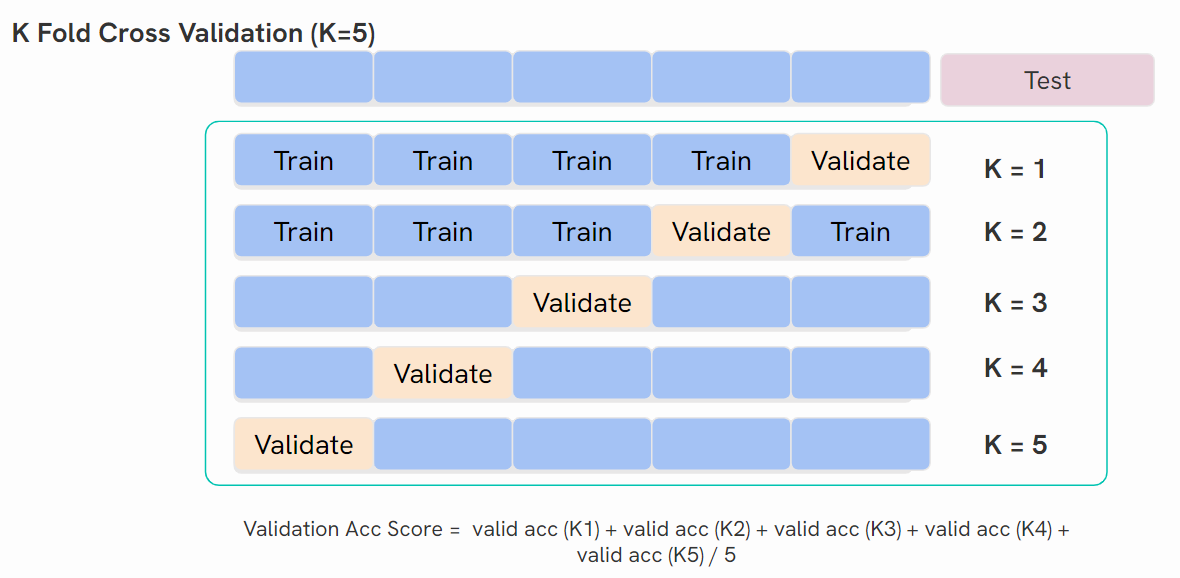
\includegraphics[width=1\linewidth]{graphics//chapter3/k fold.png}
    \caption{K Fold Cross Validation}
    \label{fig:k-fold}
\end{figure}

In each set (fold) training and the test would be performed precisely once during this entire process. It helps us to avoid overfitting. As we know when a model is trained using all of the data in a single short and give the best performance accuracy. To resist this k fold cross validation in machine learning cross-validation helps us to build the model is a generalized one.

    \subsection{Stratified K fold validation}
    Stratified K-Fold Cross-Validation is a variation of K-Fold Cross-Validation that ensures each fold maintains the same proportion of observations for each target class as the complete dataset. This is especially crucial for datasets where one class might be heavily underrepresented.

    \begin{figure}
        \centering
        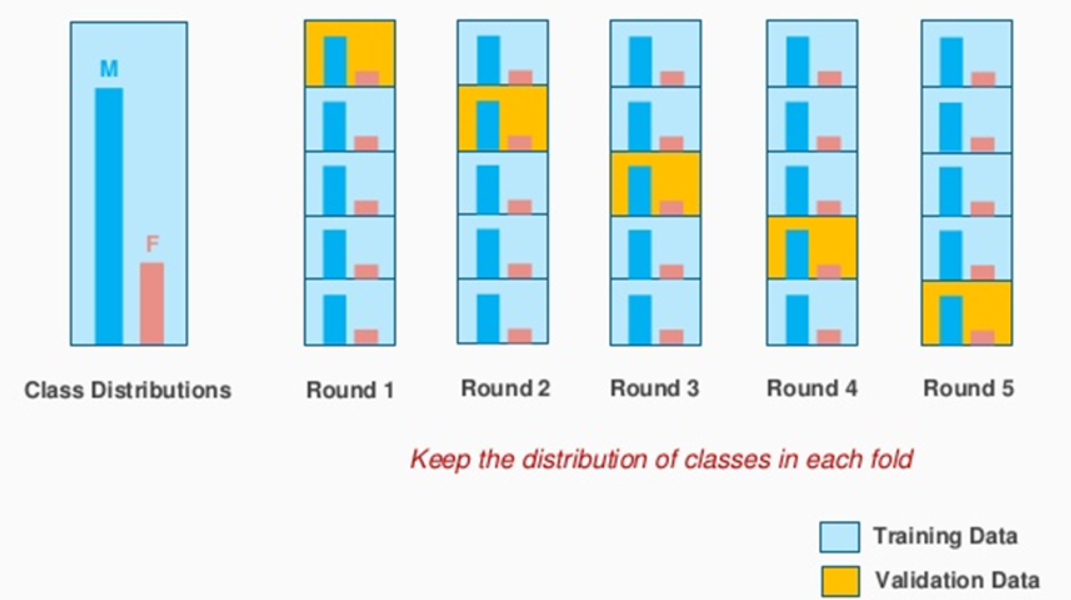
\includegraphics[width=0.75\linewidth]{graphics//chapter3/stratified k fold.png}
        \caption{Stratified K Fold Validation, Source: \cite{WEBSITE:skfold-credit}}
        \label{fig:stratified-k-fold}
    \end{figure}
    
% \section{Hyperparameter Tuning}
% Hyperparameter tuning is the process of selecting the optimal values for a machine learning model’s hyperparameters. Hyperparameters are settings that control the learning process of the model, such as the learning rate, the number of neurons in a neural network, or the kernel size in a support vector machine. The goal of hyperparameter tuning is to find the values that lead to the best performance on a given task.
%     \subsection{Grid Search}
%     \begin{figure}
%         \centering
%         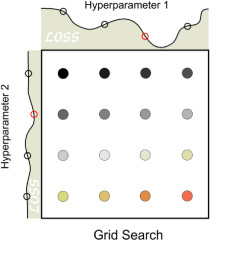
\includegraphics[width=0.5\linewidth]{graphics//chapter3/grid search.png}
%         \caption{Grid Search}
%         \label{fig:grid-search}
%     \end{figure}
%     Grid search fits the model using all possible combinations after creating a grid of potential discrete hyperparameter values. Each set's model performance is then logged and then a combination that produces the best results is chosen. This approach is called GridSearchCV, because it searches for the best set of hyperparameters from a grid of hyperparameters values. 

% \section{Batch Normalisation}
% Batch normalization is a method used to make training of artificial neural networks faster and more stable through normalization of the layers' inputs by re-centering and re-scaling.
% While the effect of batch normalization is evident, the reasons behind its effectiveness remain under discussion. It was believed that it can mitigate the problem of internal covariate shift, where parameter initialization and changes in the distribution of the inputs of each layer affect the learning rate of the network.

% \begin{figure}
%     \centering
%     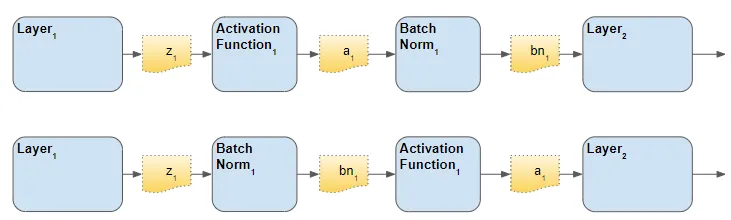
\includegraphics[width=1\linewidth]{graphics//chapter3/batch norm.png}
%     \caption{Batch Normalisation used in Neural Network Model}
%     \label{fig:batch-norm}
% \end{figure}

% \section{Dropout in Neural Network}
% Dropout is a technique used in neural networks to improve model performance and reduce overfitting. It works by randomly "dropping out" (setting to zero) a certain percentage of input and hidden units during the training process. By doing so, it helps the model generalize better and reduces the reliance on specific units, making the model more robust and less likely to overfit the training data.
% \par \vspace{1em}
% \begin{figure}
%     \centering
%     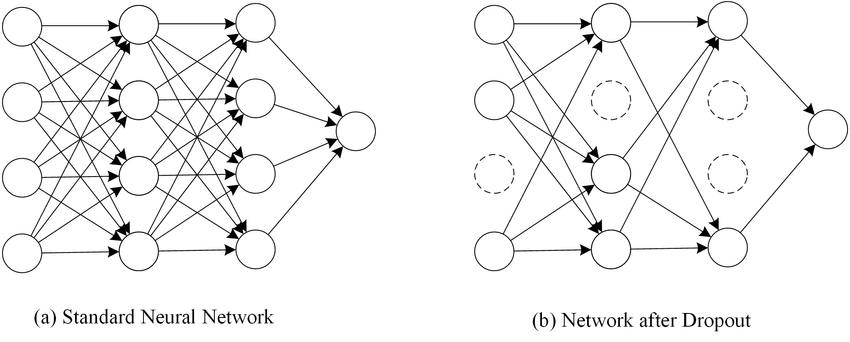
\includegraphics[width=1\linewidth]{graphics//chapter3/dropout.png}
%     \caption{Dropout}
%     \label{fig:dropout}
% \end{figure}
% During each training iteration, dropout randomly selects a fraction of the input and hidden units to be "dropped out" or set to zero. The fraction of units to be dropped out is a hyperparameter that can be tuned. This process helps prevent the neural network from relying too heavily on specific units and encourages the network to learn more robust and general features. Dropout effectively creates an ensemble of multiple subnetworks that share parameters, leading to improved generalization and reducing the risk of overfitting.
% \par \vspace{1em}
% Dropout is important because it helps address the overfitting problem in neural networks. Overfitting occurs when the model performs well on the training data but fails to generalize to unseen data. By randomly dropping out units, dropout forces the network to learn more redundant representations and prevents it from relying too heavily on specific units. This regularization technique improves the network's ability to generalize and perform well on unseen data.

% \newpage